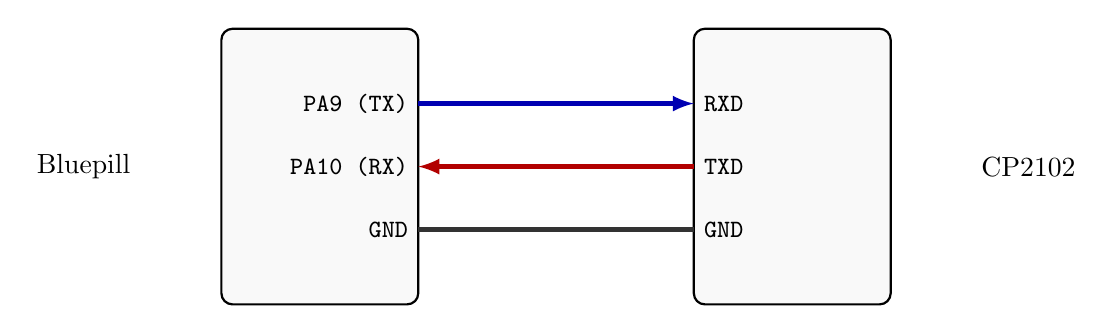
\begin{tikzpicture}[
    >=latex, 
    thick,
    box/.style={draw, rectangle, minimum height=3.5cm, minimum width=2.5cm, align=center, fill=gray!5, rounded corners},
    pinlabel/.style={font=\ttfamily\small}
]
  
  % Nodo BluePill
  \node[box] (bp) at (0,0) {};
  \node[] (lab1a) at (-3,0) {Bluepill};
  
  % Pines en la BluePill
  \node[anchor=east, pinlabel] at (1.25, 0.8)  (bp_tx)  {PA9 (TX) };
  \node[anchor=east, pinlabel] at (1.25, 0.0)  (bp_rx)  {PA10 (RX)};
  \node[anchor=east, pinlabel] at (1.25, -0.8) (bp_gnd) {GND      };
  
  % Nodo Conversor USB-UART
  \node[box] (conv) at (6,0) {};
  \node[] (lab1b) at (9,0) {CP2102};
  
  % Pines en el Conversor
  \node[anchor=west, pinlabel] at (4.75, 0.8)  (conv_rx)  { RXD};
  \node[anchor=west, pinlabel] at (4.75, 0.0)  (conv_tx)  { TXD};
  \node[anchor=west, pinlabel] at (4.75, -0.8) (conv_gnd) { GND};
  
  % Conexiones con flechas y colores
  \draw[->, color=blue!70!black, ultra thick] (1.25, 0.8) -- (4.75, 0.8);
  \draw[<-, color=red!70!black, ultra thick] (1.25, 0.0) -- (4.75, 0.0);
  \draw[-, color=black!80, ultra thick] (1.25, -0.8) -- (4.75, -0.8);
  
\end{tikzpicture}
